\documentclass[11pt]{asaproc}\usepackage[]{graphicx}\usepackage[]{color}
%% maxwidth is the original width if it is less than linewidth
%% otherwise use linewidth (to make sure the graphics do not exceed the margin)
\makeatletter
\def\maxwidth{ %
  \ifdim\Gin@nat@width>\linewidth
    \linewidth
  \else
    \Gin@nat@width
  \fi
}
\makeatother

\definecolor{fgcolor}{rgb}{0.345, 0.345, 0.345}
\newcommand{\hlnum}[1]{\textcolor[rgb]{0.686,0.059,0.569}{#1}}%
\newcommand{\hlstr}[1]{\textcolor[rgb]{0.192,0.494,0.8}{#1}}%
\newcommand{\hlcom}[1]{\textcolor[rgb]{0.678,0.584,0.686}{\textit{#1}}}%
\newcommand{\hlopt}[1]{\textcolor[rgb]{0,0,0}{#1}}%
\newcommand{\hlstd}[1]{\textcolor[rgb]{0.345,0.345,0.345}{#1}}%
\newcommand{\hlkwa}[1]{\textcolor[rgb]{0.161,0.373,0.58}{\textbf{#1}}}%
\newcommand{\hlkwb}[1]{\textcolor[rgb]{0.69,0.353,0.396}{#1}}%
\newcommand{\hlkwc}[1]{\textcolor[rgb]{0.333,0.667,0.333}{#1}}%
\newcommand{\hlkwd}[1]{\textcolor[rgb]{0.737,0.353,0.396}{\textbf{#1}}}%
\let\hlipl\hlkwb

\usepackage{framed}
\makeatletter
\newenvironment{kframe}{%
 \def\at@end@of@kframe{}%
 \ifinner\ifhmode%
  \def\at@end@of@kframe{\end{minipage}}%
  \begin{minipage}{\columnwidth}%
 \fi\fi%
 \def\FrameCommand##1{\hskip\@totalleftmargin \hskip-\fboxsep
 \colorbox{shadecolor}{##1}\hskip-\fboxsep
     % There is no \\@totalrightmargin, so:
     \hskip-\linewidth \hskip-\@totalleftmargin \hskip\columnwidth}%
 \MakeFramed {\advance\hsize-\width
   \@totalleftmargin\z@ \linewidth\hsize
   \@setminipage}}%
 {\par\unskip\endMakeFramed%
 \at@end@of@kframe}
\makeatother

\definecolor{shadecolor}{rgb}{.97, .97, .97}
\definecolor{messagecolor}{rgb}{0, 0, 0}
\definecolor{warningcolor}{rgb}{1, 0, 1}
\definecolor{errorcolor}{rgb}{1, 0, 0}
\newenvironment{knitrout}{}{} % an empty environment to be redefined in TeX

\usepackage{alltt}

\usepackage{graphicx}
\usepackage{natbib}
\usepackage[hyphens]{url}
\usepackage{color}
\usepackage{times}
\usepackage{verbatim}
%\usepackage{enumitem}
\usepackage[hidelinks,breaklinks=true]{hyperref}


\renewcommand\labelenumi{(\roman{enumi})}
\renewcommand\theenumi\labelenumi

\title{Interactive Uncertainty Quantification Visualization: Project Proposal}

\author{Matthew Isaac \thanks{Department of Mathematics and Statistics, Utah State University, Logan, UT 84322--3900, USA. 
E-mail: \url{matt.isaac@aggiemail.usu.edu}}
}
\IfFileExists{upquote.sty}{\usepackage{upquote}}{}
\begin{document}

\renewcommand{\topfraction}{1.0}
\renewcommand{\bottomfraction}{1.0}
\renewcommand{\textfraction}{0.0}
\renewcommand{\floatpagefraction}{1.0}
\renewcommand{\dbltopfraction}{1.0}


\maketitle

%\begin{abstract}
%Abstract needed for proposal?
%\end{abstract}

%\begin{keywords}Uncertainty Quantification; Visualization; Interactive; {\tt shiny} R Package
%\end{keywords}


%%%%%%%%%%%%%%%%%%%%%%%%%
\section{Introduction}
\label{Introduction}
%%%%%%%%%%%%%%%%%%%%%%%%%

Uncertainty quantification is a methodological framework used with some frequency in engineering analysis \citep{EW2018}. It is used to understand how variability  within the parameters (i.e. inputs) to some system impact the end state of that system. Engineering analysts use uncertainty quantification to assess and find the balance between design sufficiency and design efficiency. This is particularly important in fields where large-scale prototypes, testing, and data collection are extremely expensive. Engineers in these types of applications are increasingly relying on computational simulations to assess system designs.

In the following paper, I propose to implement an interactive tool to visualize uncertainty quantification results. The outline of this proposal will proceed as follows: In Section~\ref{UQOverview}, I will give a brief overview of uncertainty quantification. In Section~\ref{Implementation}, I will describe the features I propose to implement as part of this visualization tool. In Section~\ref{Packages}, I will indicate which {\tt R} packages and methods are anticipated as being necessary for the implementation.

%%%%%%%%%%%%%%%%%%%%%%%%%
\section{Uncertainty Quantification Overview}  
\label{UQOverview}
%%%%%%%%%%%%%%%%%%%%%%%%%

The following description of the uncertainty quantification algorithm is adapted from \cite{EW2018}. First, a few terms and definitions will be described. 

\begin{description}
\item[system response quantity (SRQ):] A parameter of particular interest directly related to the engineering system in question. The SRQ is the output (i.e. prediction) from the engineering model.
\item[engineering model:] A mathematical model that defines the relationship between the parameters (model inputs) and SRQ (model output). 
\item[aleatory uncertainty:] Uncertainty resulting from randomness inherent to a given parameter. Gaining more knowledge about the parameter will not reduce the uncertainty of the parameter. 
\item[epistemic uncertainty:] Uncertainty resulting from a lack of knowledge about a given parameter. Gaining more knowledge about the parameter could reduce the uncertainty of the parameter. 
\end{description}

The first step of uncertainty quantification is to identify sources of uncertainty (model parameters) and classify them as either aleatory or epistemic. This classification process has been somewhate debated in literature \citep{KD2009}, and will not be discussed as it is outside the scope of this project. Once these uncertainties related to the model parameters have been identified and classified as aleatory or epistemic, the uncertainty for each parameter must somehow be described. Traditionally, epistemic uncertainties have been described by an interval over which any value in the interval is equally likely, while aleatory uncertainties have been assigned probability distributions. Some more recent publications \citep{EW2018} propose that all uncertainties, aleatory or epistemic, be described using probability distributions. This debate will not be discussed here as it is, again, outside the scope of this project. Once these distributions and/or intervals have all been assigned, they are carried through the model using Monte Carlo techniques.

Let $m$ denote the number of iterations of an outer for loop, and let $n$ denote the number of iterations in an inner for loop. In the outer for loop, values for the epistemic uncertainty parameters are selected randomly from the intervals/distributions assigned. Upon entering the inner loop, values for the aleatory uncertainty parameters are randomly chosen from the distributions assigned. The values chosen for the parameters in both the outer loop and the inner loop are then used as inputs in the engineering model to calculate a value for the SRQ. This value is stored and the inner loop continues running for the rest of the $n-1$ iterations. All of the $n$ SRQ values calculated from the $n$ iterations of the inner loop are used to calculate an empirical cumulative distribution function (CDF) of SRQ values and the CDF is stored. The outer loop then begins its second iteration, and new values for the empirical uncertainty parameters are chosen. The inner loop then runs another $n$ iterations, producing another CDF. This process continues until the outer loop has run all of its $m$ iterations. 

At this point, there will be $m$ empirical CDFs that have been calculated, representing various possible realized values of the SRQ. These CDFs can then be plotted and interpreted. \cite{EW2018} suggests constructing a ``P-box". This P-box is found by calculating a lower percentile (e.g. the 5th percentile) and an upper percentile (e.g. the 95th percentile) of the CDF ensemble. This P-box can then be interpreted in several ways, including (1) selecting a SRQ value and extracting a probability interval, and (2) selecting a probability value and extracting an SRQ interval.

%%%%%%%%%%%%%%%%%%%%%%%%%
\section{Implementation}  
\label{Implementation}
%%%%%%%%%%%%%%%%%%%%%%%%%

I propose to implement an interactive visualization tool to assist analysts in visualizing and interpreting results from an uncertainty quantification analysis as described in Section~\ref{UQOverview}. Since the actual uncertainty quantification analysis can likely be carried out with greater speed and computational power elsewhere, this implementation will not include the Monte Carlo portion of the implementation described in Section~\ref{UQOverview}. Users will begin by uploading a {\tt .csv} file, which should contain the ensemble of CDFs generated from the Monte Carlo process. I also plan to include several sample data sets that users can select and use to experiment with. The CDFs will be plotted with the x-axis displaying the SRQ values and the y-axis displaying the probability values. Once the ensemble of CDFs have been uploaded, or a sample data set selected, users will be able to interact with the visualization in various ways, including:

\begin{itemize}
\item toggle P-box on/off
\item select percentiles to be used in P-box calculation
\item toggle CDF ensemble on/off (so only P-box is displayed)
\item select level of transparency for CDF ensemble
\item input a probability value and extract (display) an SRQ interval
\item input a SRQ value and extract (display) a probability interval
\item download and save the visualization in its current state
\end{itemize}

The prototype layout is shown in a diagram in Figure~\ref{AppLayout}. The web application will consist of a main pane which will display the graphical visualization. A control panel below the plot will hold the controls (toggle buttons, check boxes, sliders, {\tt .csv} upload) to be used when interacting with the visualization. 

\begin{figure}[t]
\begin{center} 
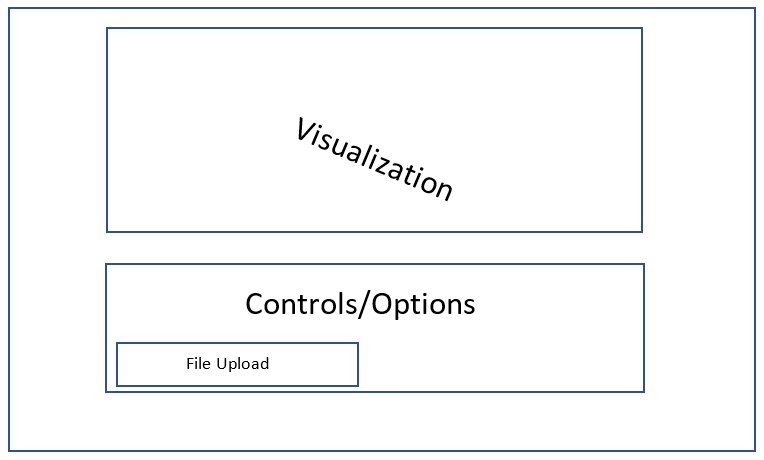
\includegraphics[height=6cm,width=10cm]{figures2/app_layout.png}
\end{center} 
\caption{\label{AppLayout}Proposed layout of web application.}
\end{figure}

%%%%%%%%%%%%%%%%%%%%%%%%%
\section{{\tt R} Packages and Methods}  
\label{Packages}
%%%%%%%%%%%%%%%%%%%%%%%%%

I anticipate the following packages and methods being useful and/or necessary in carrying out this implementation.

\subsection{{\tt dplyr}}
The {\tt dplyr} package \citep{DPLYR} is a data-wrangling and manipulation package implemented in {\tt R}. The methods in this package will be used to manage and manipulate the CDFs from the {\tt .csv} file into a convenient format for plotting. 

\subsection{{\tt shiny}}
The {\tt shiny} package and framework \citep{SHINY} will be the backbone of this project. {\tt shiny} provides a way to create and deploy web applications through RStudio \citep{RSTUDIO}. It also contains the implementations for all user-interface components (toggle buttons, check boxes, numeric inputs, sliders, etc.). A package such as {\tt shinydashboard} \citep{DASH} may also be used as a aesthetic wrapper around the {\tt shiny} framework. This package will be used to create and deploy the actual web application. The controls in the we app will be made from the user-interface components in this package. 

\subsection{{\tt ggplot2}}
The plotting functionality of the {\tt ggplot2} package \citep{GGPLOT} will be used to generate the actual visualization and to add, remove, or adjust components on the plot. 

\subsection{{\tt plotly}}
The {\tt plotly} package \citep{PLOTLY} will be used to add additional interactive capabilities to the plot. {\tt plotly} includes a method called {\tt ggplotly()} which will be used to convert the {\tt ggplot} plot object to a {\tt plotly} plot object. The {\tt plotly} plots contain options to zoom in and out on a plot, show plot values when hovering with mouse, download and save a {\tt .png} version of the plot, and download and save an interactive {\tt html} version of the plot. 

\vspace{5mm}

Since the existing {\tt R} packages already implement most of the tools I will need to generate the plot and implement user interface elements, my primary objective on this project will be to seamlessly combine elements from the packages above (particularly the {\tt shiny}, {\tt ggplot2}, and {\tt plotly} packages) to create a user-friendly interactive visualization tool. 

\bibliographystyle{elsarticle-harv}
% modified to add 
%     \itemsep=0pt
% to 2nd line of file paper.bbl

\bibliography{references2}


\end{document}
